\documentclass[a4paper,12pt]{article}

\usepackage{geometry}       % Required for page layout.
\usepackage{hyperref}       % Required for hyperlinks.
\usepackage{graphicx}       % Required for figures.
\usepackage{subfig}         % Required for minipages.
% \usepackage{caption}
% \usepackage{subcaption}
\usepackage{placeins}
\usepackage{float}

\usepackage{amsmath}

\newgeometry{vmargin={25.4mm}, hmargin={27mm,27mm}}
\setlength\parindent{0pt}   % Disable paragraph indent.

\title{Project 4: Electrostatics}
\author{
  Elias Rilegård\\
  \texttt{eliasril@kth.se}
}

\begin{document}
\maketitle

\section*{Exercise 4.1: Laplace's Equation}

This exercise revolves around determining the potential $V(x,y)$ in a square region with a length $L = 10$.

\subsection*{Part a}

The potential $V$ at a point $(x, y)$ can be approximated as

\begin{equation*}
  V(x, y) \approx \frac{1}{4} \biggl[ V(x + \Delta x, y) + V(x - \Delta x, y) + V(x, y + \Delta y) + V(x, y - \Delta y) \biggr]
\end{equation*}

To begin, we let $\Delta x = \Delta y = 1$, ie we only look at the potential at points $(x,y)$ where $x$ and $y$ are
both integers. Before running the relaxation, the task was to estimate/guess the shape/structure of the potential and
to set the initial potential $10 \%$ lower than the exact answer. Since the potential is given ($V = 10$) at all edges
and there are no charges within the region, we can conclude that $V$ must be constant in the region. This can be
backed up by running a quick simulation and relaxing it. 

\begin{figure}[!ht]
  \centering
  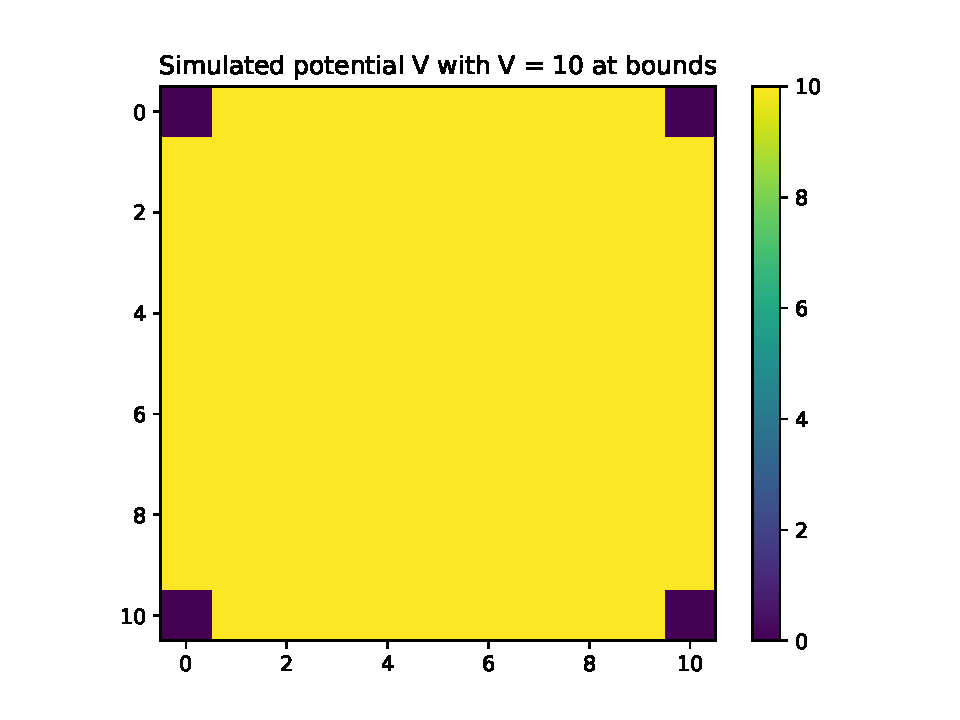
\includegraphics[scale=0.49]{img/4_1a_simulated_V.pdf}
\end{figure}

Do note that the potential at the four corners is irrelevant due to them not affecting the calculations of any point.
(The only points which they can affect are also on the edge, which are fixed in this case.) From the animation it's
clear that it's the center point that takes the longest to stabilize. If we define the absolute error $\epsilon$ and
relative error $\eta$ as

\begin{equation*}
  \epsilon = | v - v_{approx} |,\quad \eta = \frac{\epsilon}{|v|}
\end{equation*}

where $v$ is the correct value and $v_{approx}$ is the approximation of the value (which is what the relaxation
algorithm does), we can graph the relative error for the center cell against the number of relaxation steps taken:

\begin{figure}[!ht]
  \centering
  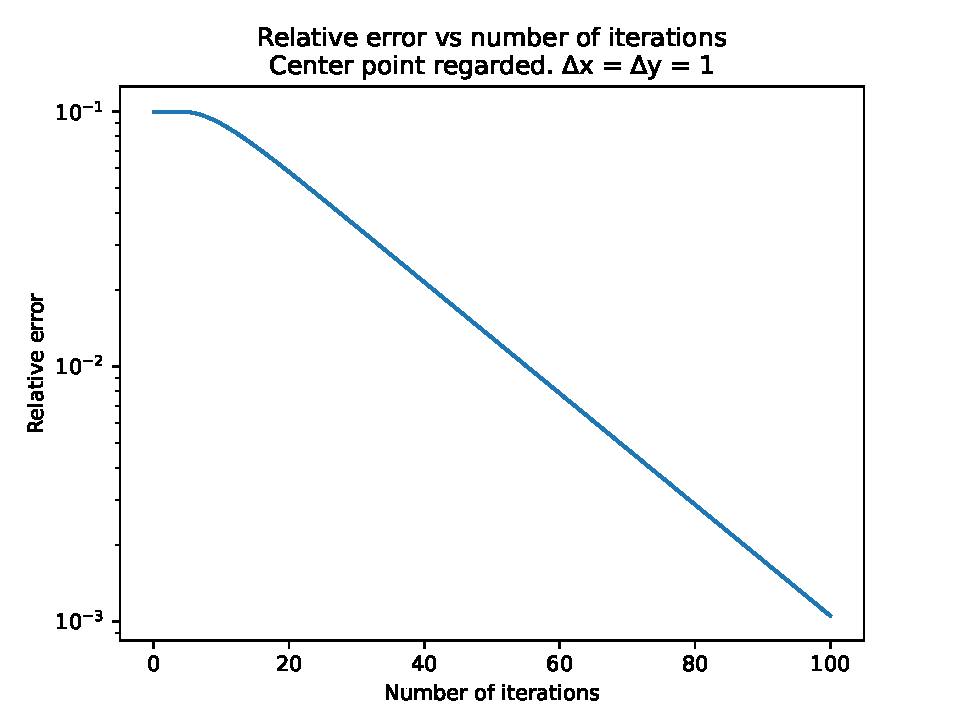
\includegraphics[scale=0.49]{img/4_1a_errorvsn_default.pdf}
\end{figure}

Here we note that the flat part in the beginning is caused due to the way the relaxation algorithm works; initially
the neighbors around the cell all have the same value. It's only when the neighbors start updating that the cell gets
a chance to update its own value. As soon as the update "wave" has reached the center, we see a steady decline in
the relative error as we take more relaxation steps. In order to reach $\eta = 1\% = 10^{-2}$, we need $56$ iterations
at the very least. If we decrease $\Delta x$ and $\Delta y$ to $0.5$ (meaning we're now dealing with a grid with
double the side length) and repeat the process, the following graph is obtained:

\begin{figure}[!ht]
  \centering
  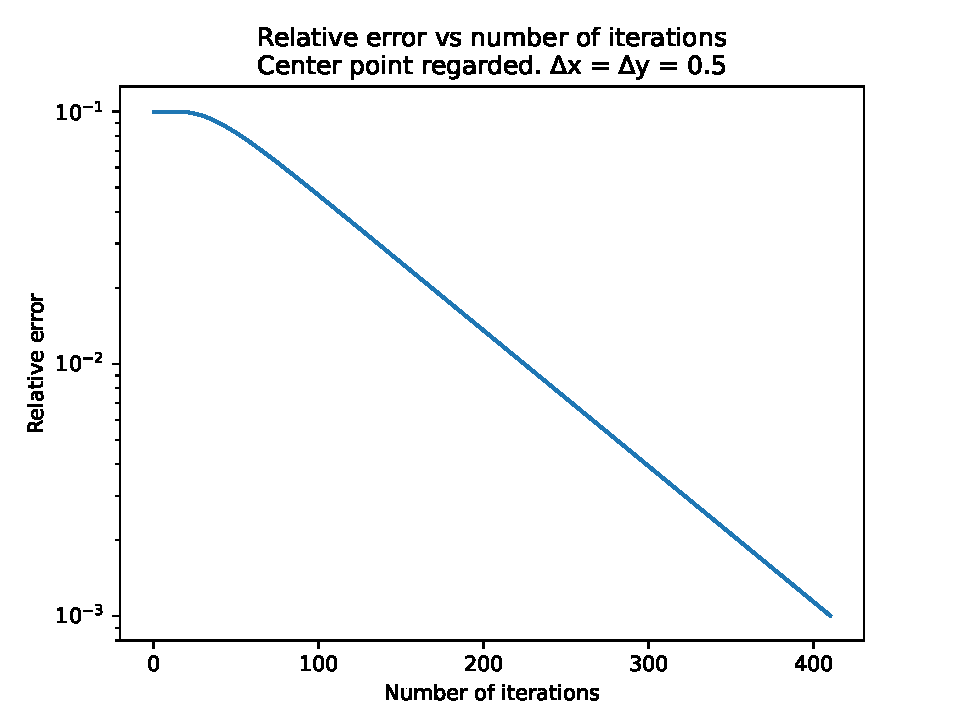
\includegraphics[scale=0.49]{img/4_1a_errorvsn_smallerd.pdf}
\end{figure}

We notice the same phenomenon happening in the beginning where the relative error takes a few iterations before it
starts to decrease. The slope is more or less the same as for when $\Delta x = \Delta y = 1$. Here it takes a minimum
of $225$ iterations to reach $\eta = 1\%$.

\subsection*{Part b}

Now we consider the same geometry as in Part a, but we set the initial potential at the interior sites equal to $0$,
except for the center, whose potential is set to $4$. Since the potential at the boundary is still the same and the
potential at every point is updated as a function of its neighbors, we can conclude that the potential will evolve to
the same state as in Part a. Plotting the relative error for the center point this time yields the following:

\begin{figure}[!ht]
  \centering
  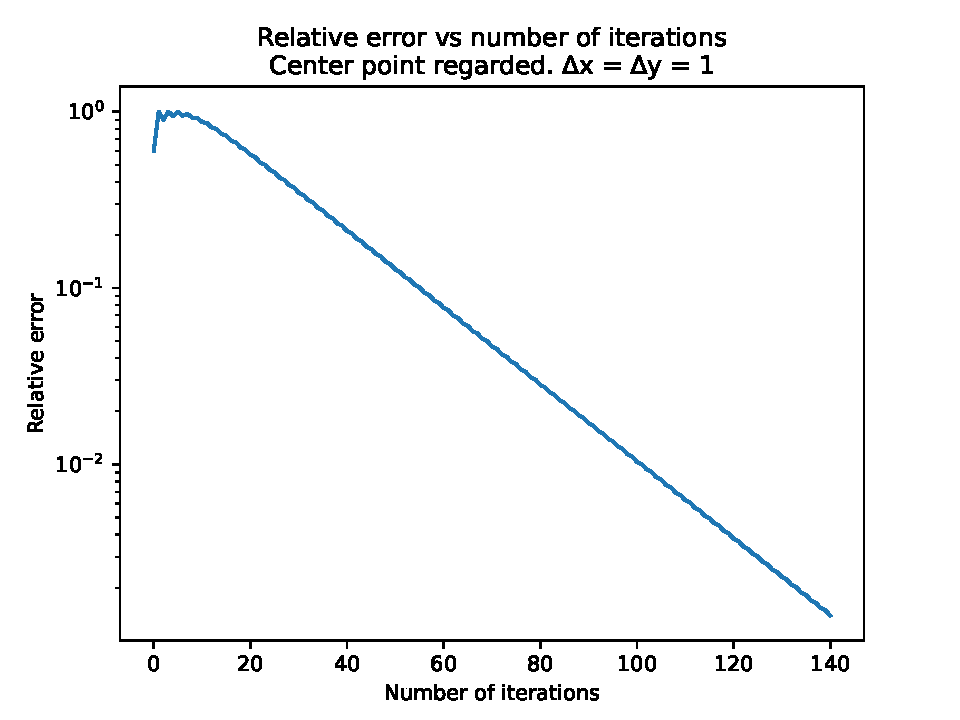
\includegraphics[scale=0.49]{img/4_1b_errorvsn.pdf}
\end{figure}

What's immediately apparent is that due to how the relaxation method works, the relative error stats slightly lower
and shoots back up to $1$ immediately in the following iteration, since the average of the four neighbors around the
center is $0$. In the following iterations, the relative error oscillates slightly (applies for all points, not just
the center one) as a remnant of the lone potential in the center, similar to how rings on water form after a stone is
dropped in. Since the algorithm requires fixed boundary conditions, the final state is more or less unambiguously defined
regardless of the initial guess. Here it takes $102$ iterations to reach $\eta = 1\%$, compared to $56$ in the
corresponding case in Part a where we set $V = 9$ initially. Using a good guess of how $V$ looks can thus cut the
number of required iterations to reach a desired $\eta$ roughly in half.

\subsection*{Part c}

Modifying the boundary potential to be $[10, 5, 10, 5]$ respectively, the potential can be calculated using a
simulation, yielding the following. Note that the values in the corners have been modified to increase the contrast
in the rest of the graph.

\begin{figure}[!ht]
  \centering
  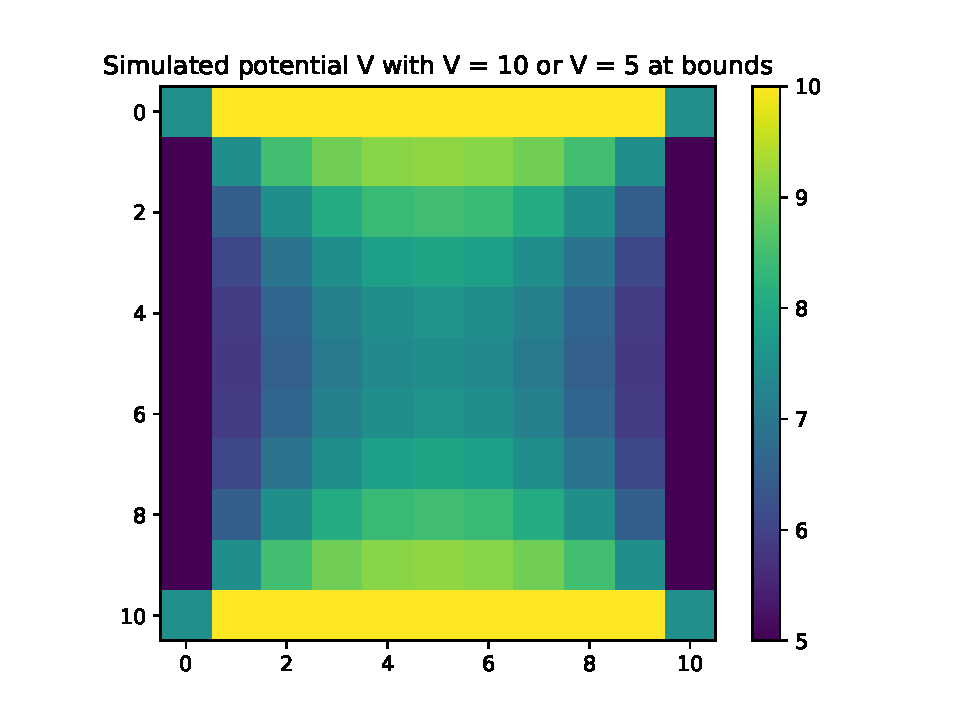
\includegraphics[scale=0.49]{img/4_1c_simulated_105105.pdf}
\end{figure}

In order to obtain smooth equipotential surfaces (the surfaces where the potential doesn't change), a value of
$\Delta x = \Delta y = 0.1$ was used. This was purely a measure taken in order to make the plots smoother.
Sketching the equipotential surfaces after iterating to make the relative error $\eta \leq 1\%$ yields:

\begin{figure}[!ht]
  \centering
  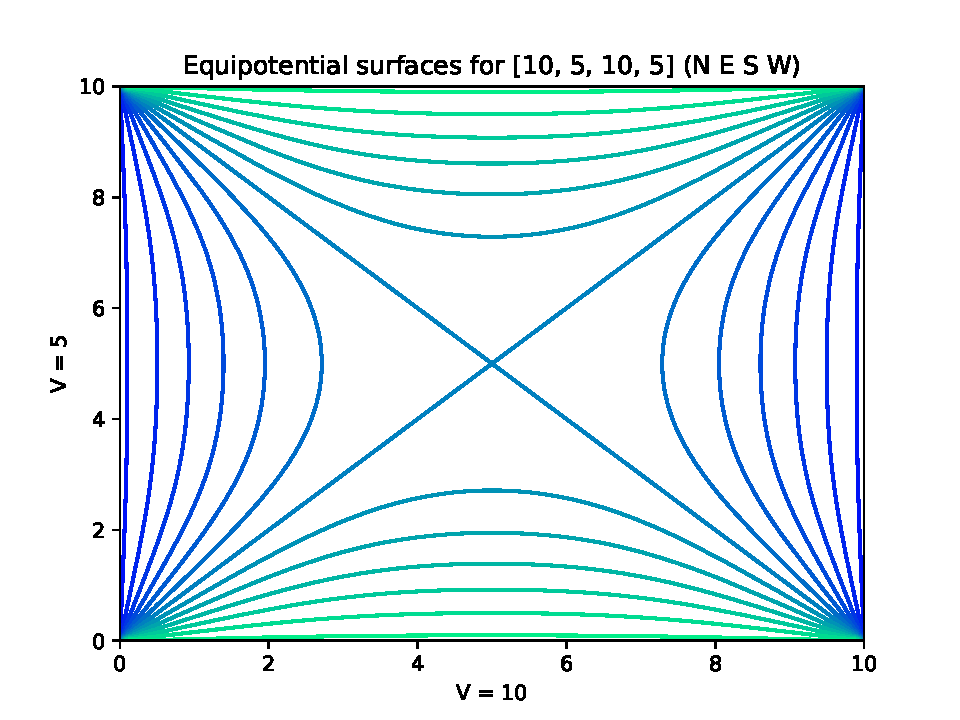
\includegraphics[scale=0.49]{img/4_1c_equipotential_510510.pdf}
\end{figure}

Comparing against the previous plot, the lines in this graph corresponds to paths where the potential (drawn as color)
is the same. Due to the symmetries of the geometry, we obtain a cross pattern in the middle and arches running close
to the edges. This makes sense since staying somewhat close to an edge should keep the potential more or less constant
and straying away from an edge allows the other edges' potential to influence. In the case where three of the
boundaries have $V = 10$ and the last one has $V = 0$, running a simulation and drawing the equipotential surfaces
(again, with $\eta \leq 1\%$) yields the following graphs.

\begin{figure}[!ht]
  \centering
  \begin{minipage}{0.49\textwidth}
    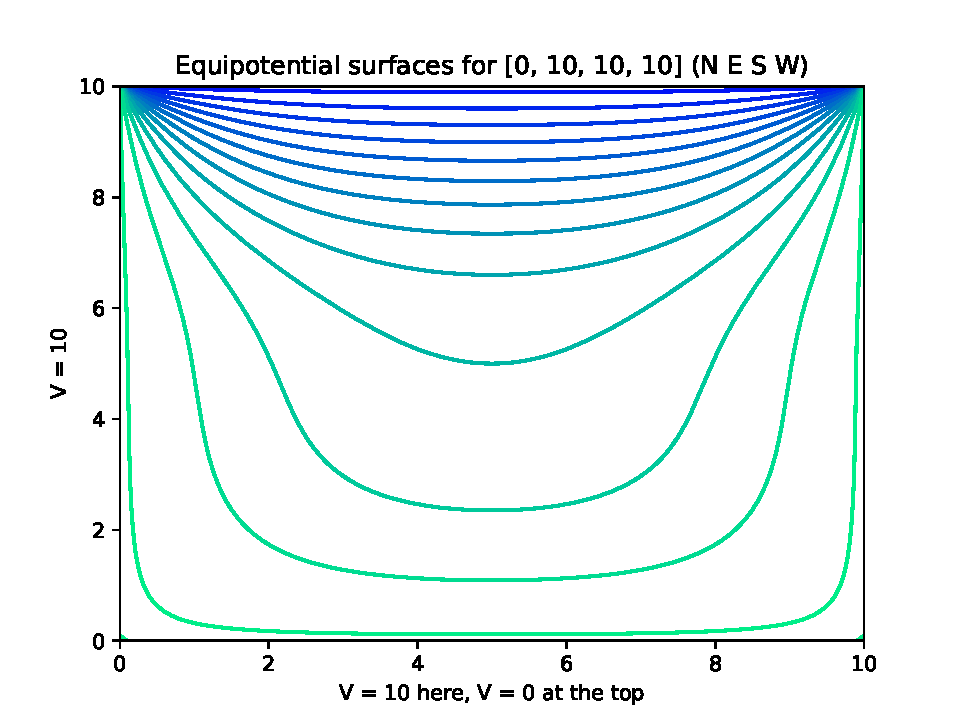
\includegraphics[width=\textwidth]{img/4_1c_equipotential_1010010.pdf}
  \end{minipage}
  \begin{minipage}{0.49\textwidth}
    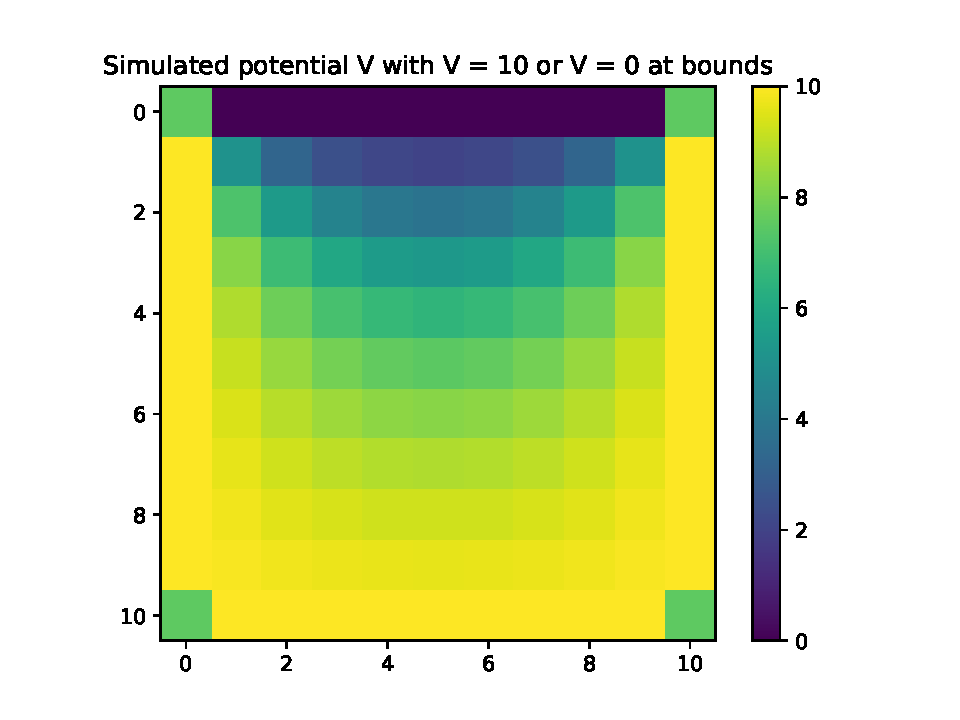
\includegraphics[width=\textwidth]{img/4_1c_simulated_1010010.pdf}
  \end{minipage}
\end{figure}

Again, it's obvious that staying close to the three edges where $V = 10$ should keep the potential more or less
constant, which is indicated by the equipotential line running close to the edges. As one drifts closer to the center
of the figure, the influence of the edge where $V = 0$ becomes more and more relevant, causing $V$ to drop, albeit
rather slowly. Approaching the north edge (where $V = 0$), the potential drops sharply.

\section*{Exercise 4.2: Gauss-Seidel Relaxation}

Gauss-Seidel Relaxation is a modified version of the relaxation algorithm where the potential of the spots is updated
immediately instead of saved before every spot is updated simultaneously. This means that the new potential of a spot
is always computed using the most recently computed potential of its nearest neighbor potentials.

\subsection*{Part a}

Modifying the program to update each spot immediately instead of simultaneously and looking at the required number
of iterations to reach $\eta = 1\%$ results in the following graph:

\begin{figure}[!ht]
  \centering
  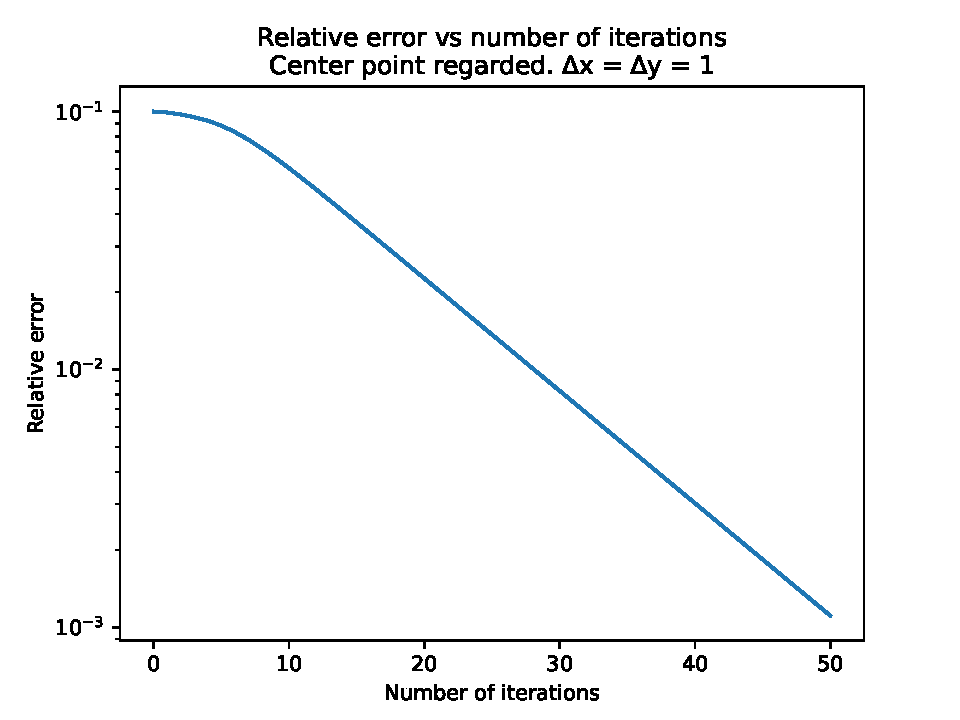
\includegraphics[scale=0.49]{img/4_2a_errorvsn_default.pdf}
\end{figure}

It's immediately apparent that the relative error immediately starts decreasing, since the updating "wave" no longer
takes any time to propagate through the grid. Comparing to the simple relaxation method we discussed in Exercise 4.1
and picking good initial values for $V$, this method cuts the number of required iterations in half again. With only
$29$ iterations required to achieve $\eta \leq 1\%$, this method performs much better than the previous ones. From a
computer science perspective, this method is superior not only because it's faster, but also because it's in-place.

\subsection*{Part b}

Imagine coloring alternating spots red and black, making the grid resemble a chess board. The task here was to
update the algorithm to comprise a single step as first computing the potential for all red spots first and then
all black spots. Plotting the relative error against the number of iterations yields:

\begin{figure}[!ht]
  \centering
  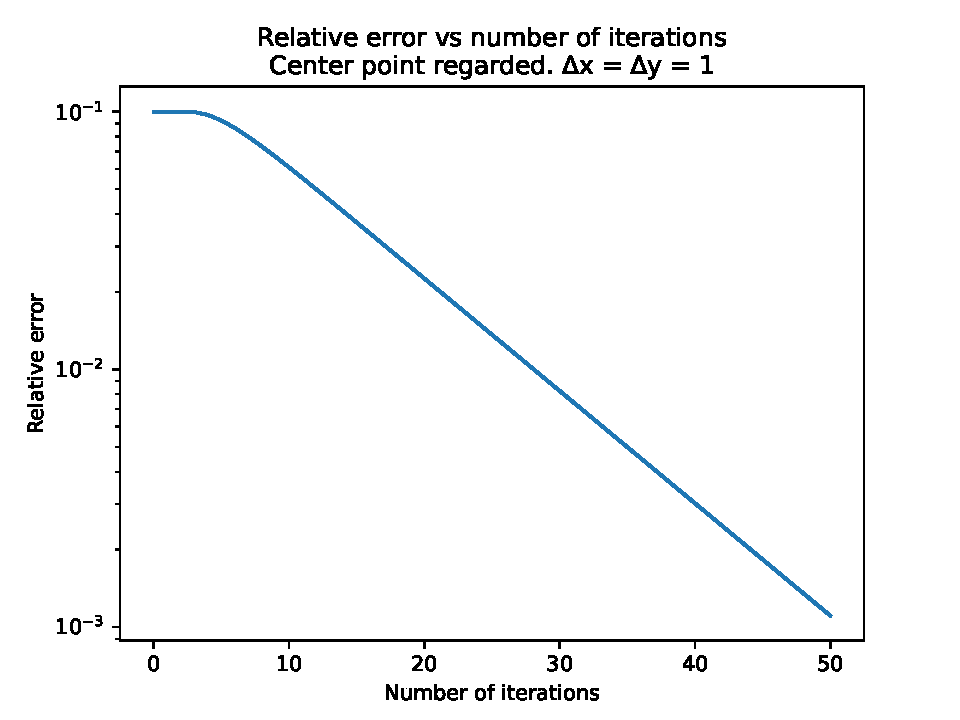
\includegraphics[scale=0.49]{img/4_2b_errorvsn_checker.pdf}
\end{figure}

Comparing against the original Gauss-Seidel relaxation method, the rate of convergence is about the same here, though
again we notice that the updating "wave" now takes a couple of iterations of propagation to reach the center. While
this might seem to make the method less attractive since it's computationally more complex to implement, the fact that
it also takes exactly $29$ iterations before $\eta \leq 1\%$ implies that the rate of convergence actually is slightly
better, due to $\eta$ not changing in the first couple of iterations.

\section*{Exercise 4.3: Random-walk solution of Laplace's Eq.}

In this geometry, the potential $V(x, y)$ can also be estimated using random walks that walk from $(x, y)$ until they
hit a boundary. The value of the potential at the point $(x, y)$ can be estimated by

\begin{equation*}
  V(x, y) = \frac{1}{n}\sum_{i = 1}^{n} V_b(i)
\end{equation*}

where $V_b(i)$ denotes the potential of the boundary that the $i$-th walk reached and $n$ is the total number of
random walks used in the estimation.

\subsection*{Part a}

Using the same square region with $[10, 5, 10, 5]$ boundary conditions, we can analyze the results of the random walk
method and compare against the relaxation method. For simplicity's sake, we pick $(x, y) = (5, 5)$ like we had in
the previous exercises. Plotting the estimated potential and the relative error against the number of walks used
results in the following graphs:

\begin{figure}[!ht]
  \centering
  \begin{minipage}{0.49\textwidth}
    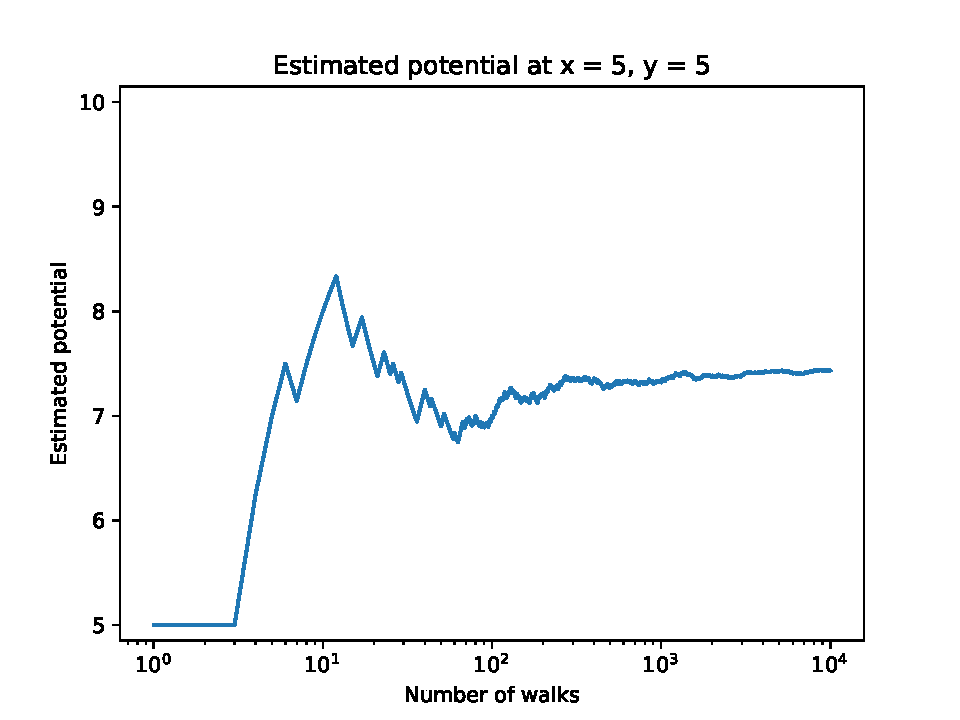
\includegraphics[width=\textwidth]{img/4_3a_V55.pdf}
  \end{minipage}
  \begin{minipage}{0.49\textwidth}
    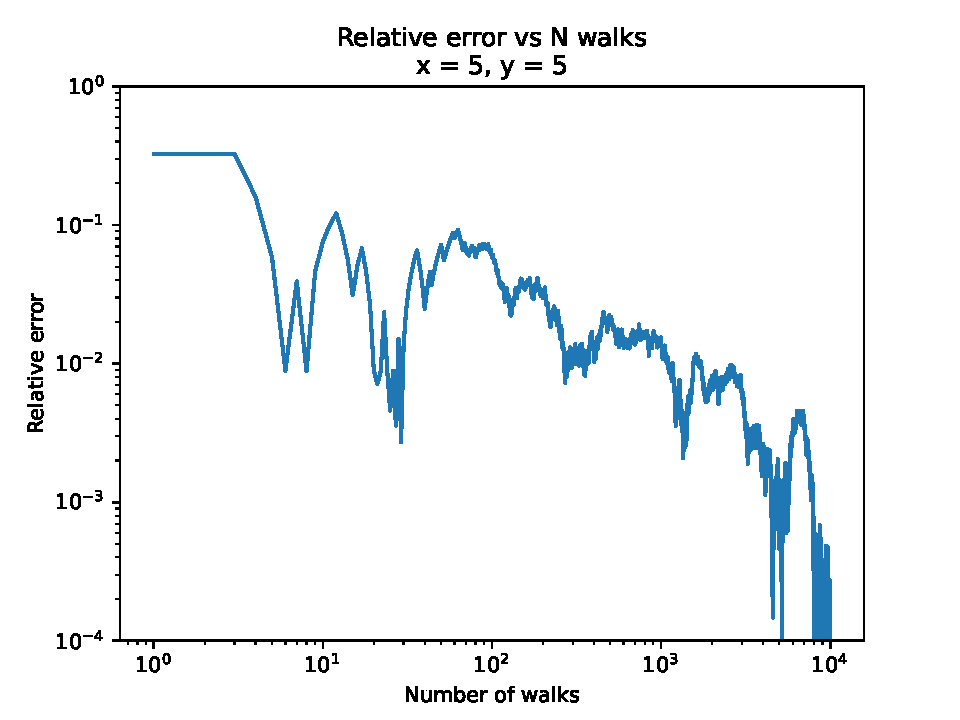
\includegraphics[width=\textwidth]{img/4_3a_E55.pdf}
  \end{minipage}
\end{figure}

While the exercise called for $N = 100$ and $N = 1000$ walks, according to these plots, $N = 1000$ might not always
be enough to guarantee $\eta \leq 1\%$. Of course, for a bigger geometry (recall that $L = 10$ in this assignment),
using more than $10^3$ walks per point to calculate might be computationally infeasible. The sudden sharp drops in
the relative error diagram can be explained by the walks sampling a ratio of the values of the boundaries that
approximates the sought value very closely. This would cause the absolute error $\epsilon$ to be tiny, which would in
turn cause the relative error $\eta$ to be small as well.

\subsection*{Part b}

Here the task was to repeat what we did in Part a for more points, not necessarily for points close to the middle
though. Choosing $(x, y)$ somewhat arbitrarily to be $(2, 5)$ and $(1, 1)$ and plotting the estimation diagrams and
the relative error diagrams respectively yields:

\begin{figure}[!ht]
  \centering
  \begin{minipage}{0.49\textwidth}
    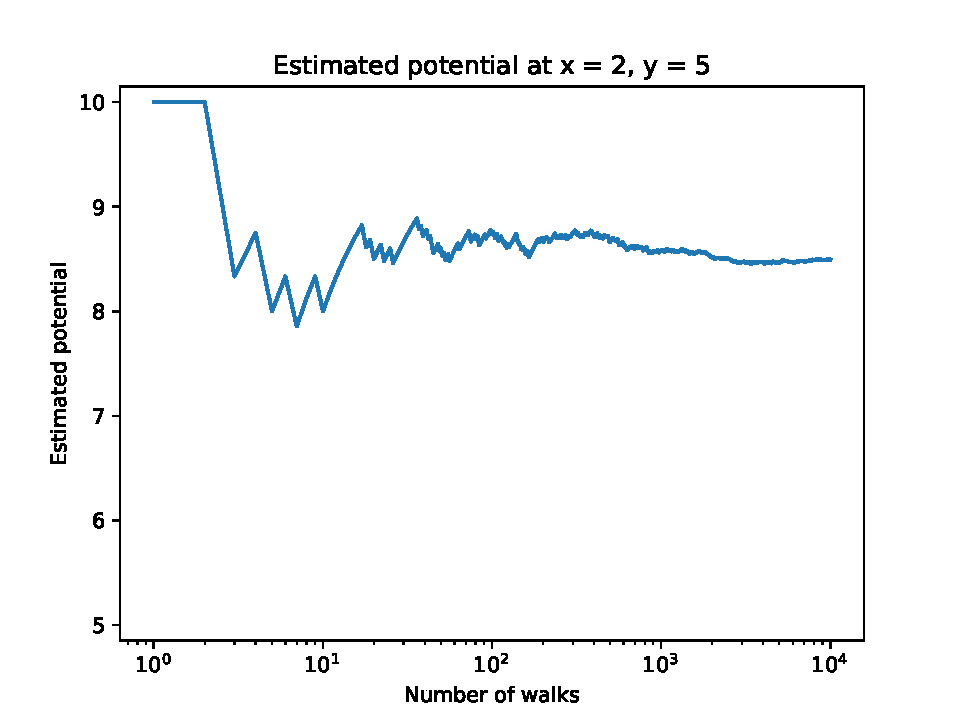
\includegraphics[width=\textwidth]{img/4_3b_1_V25.pdf}
  \end{minipage}
  \begin{minipage}{0.49\textwidth}
    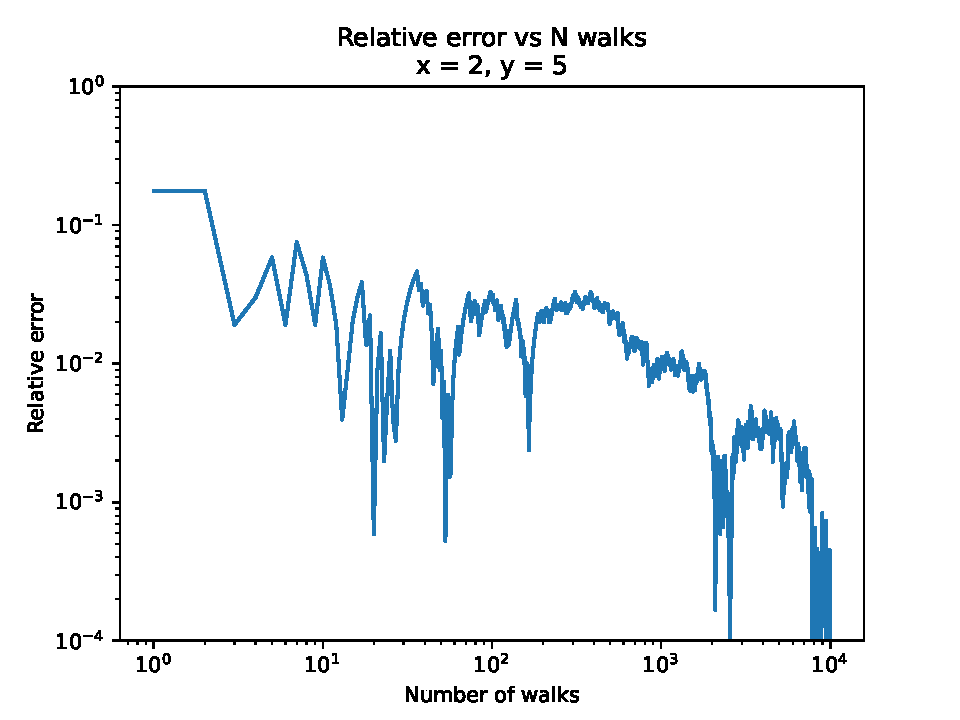
\includegraphics[width=\textwidth]{img/4_3b_1_E25.pdf}
  \end{minipage}
\end{figure}

\begin{figure}[!ht]
  \centering
  \begin{minipage}{0.49\textwidth}
    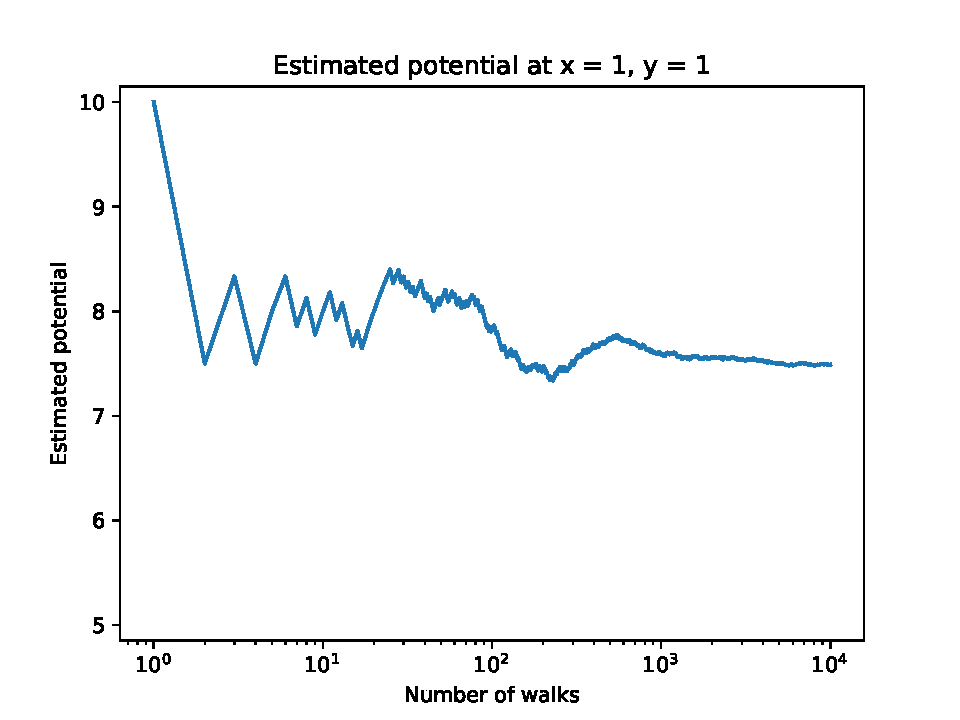
\includegraphics[width=\textwidth]{img/4_3b_2_V11.pdf}
  \end{minipage}
  \begin{minipage}{0.49\textwidth}
    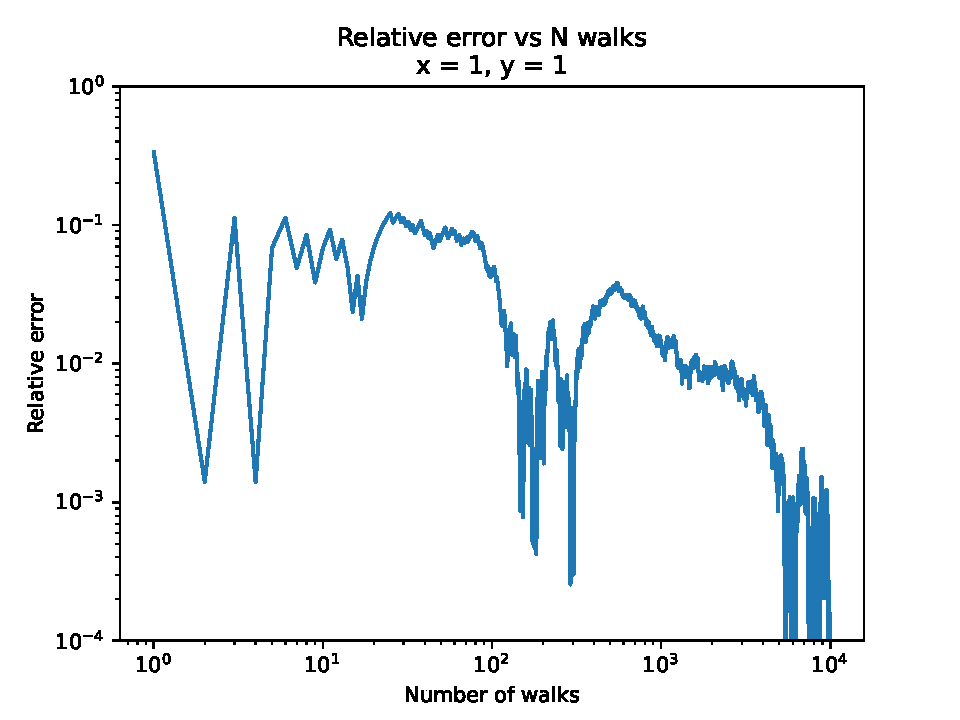
\includegraphics[width=\textwidth]{img/4_3b_2_E11.pdf}
  \end{minipage}
\end{figure}

There doesn't seem to be a clear answer when it comes to how the number of walks required for a point close to a
boundary compares to a point closer towards the middle of the geometry. If anything, \emph{more} walks are required
as the point being evaluated moves closer to the edge, but it's hard to say for certain from these graphs.

From numerical methods we can estimate the order of convergence $p$ of a function $u$ as

\begin{equation*}
  p \approx \mathrm{log}_{2}\biggl( \frac{u(h) - u(\frac{h}{2})}{u(\frac{h}{2}) - u(\frac{h}{4})} \biggr)
\end{equation*}

where $h$ here is the number of walks. While these graphs are very rough due to the randomness of the random walks,
we can estimate $p$ to be around $0.8$ for all three error plots.

\section*{Exercise 4.4: Green's Functions}

As long as the geometry of the problem remains the same, it's a waste of computation to recalculate the random walk
destination distribution every time one wants to run a simulation. Instead, we can calculate the Green's function
$G(x, y, x_b, y_b)$, which essentially is the distribution of how the boundary positions $(x_b, y_b)$ affects the
potential at $(x, y)$. The random walk algorithm is thus equivalent to the relation

\begin{equation*}
  V(x, y) = \frac{1}{n} \sum_{x_b, y_b} G(x, y, x_b, y_b) V(x_b, y_b)
\end{equation*}

where the sum is over all points on the boundary. The beauty here is that we can use the same $G$ for different
distributions of the potential $V$.

\subsection*{Part a}

The Green's function $G(x, y, x_b, y_b)$ was computed by from every point in the geometry, starting $N$ walks that
wanders out to the boundary, and recording where they land. Doing this for sufficiently large $N$ (the assignment
suggested $N \geq 200$, but to ensure reliability, $N = 10000$ was used instead) and for all starting points and
normalizing the values, we generate a distribution of how the random walks distribute over the boundary, for each
starting point $(x, y)$. This distribution is what is saved for later use.

\subsection*{Part b}

Using the Green's function generated in Part a, we can estimate the potential distribution with the boundary values
$[10, 5, 10, 5]$. Plotting the estimation yields:

\begin{figure}[!ht]
  \centering
  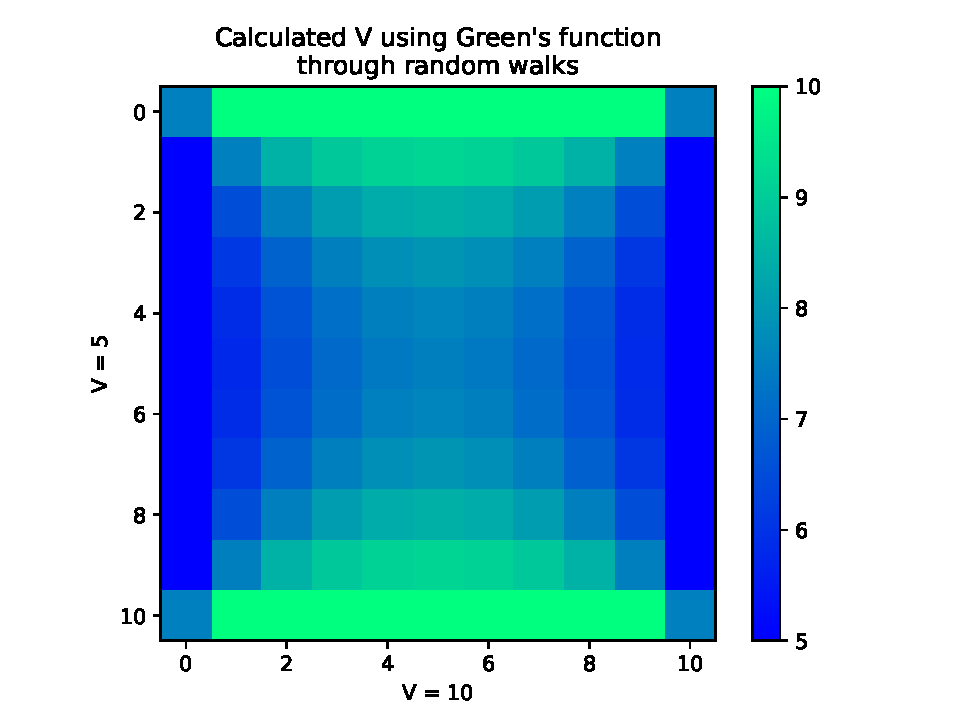
\includegraphics[scale=0.49]{img/4_4b_VfromG.pdf}
\end{figure}

This matches almost exactly what we got in Exercise 4.1, Part c. The corner values have been manually changed to
improve the contrast and clarity of the figure. Now we set five of the points' potential to $20$ and search for the
optimal placements of these points to maximize the potential of the point $(3, 5)$. Physical intuition says that
since these stronger points are $2$ to $4$ times as strong as the rest, they should be placed as close to the point
of interest as possible. This can be backed up by looking at $G(3, 5, x_b, y_b)$ for all $(x_b, y_b)$. The coordinates
which have the biggest influence matches the guess led by physical intuition. Hence we place them in a line centered
at $(0, 5)$. Plotting the estimation of the potential yields:

\begin{figure}[!ht]
  \centering
  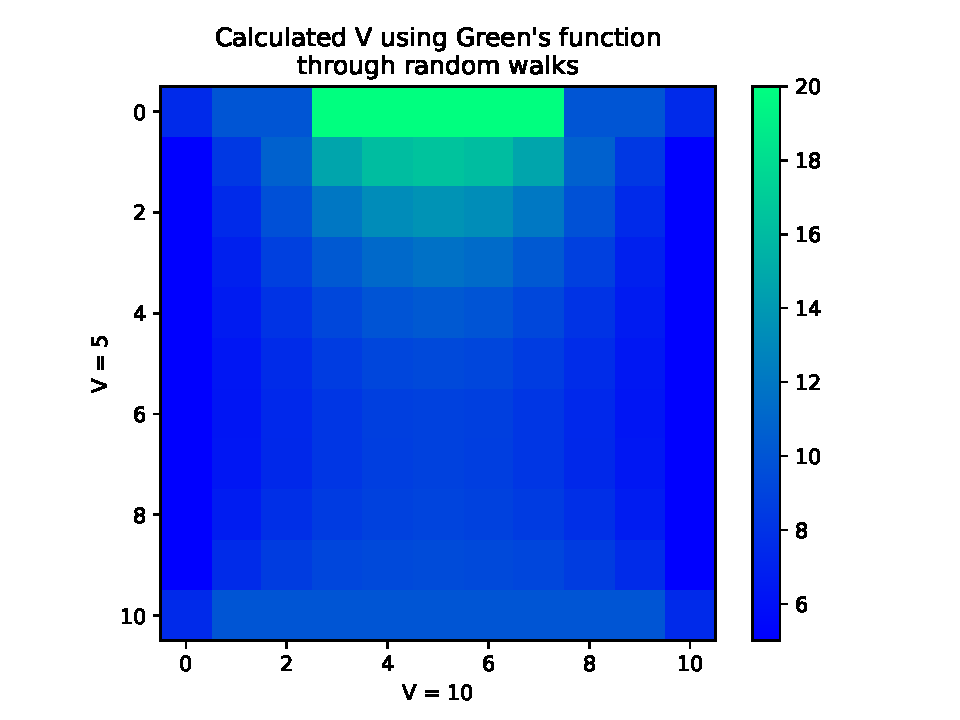
\includegraphics[scale=0.49]{img/4_4b_1_VfromG.pdf}
\end{figure}

\FloatBarrier

This configuration maximizes $V$ at the point $(3, 5)$, which results in $V(3, 5) = 11.64$. Repeating the same thought
process and analysis for the case where we want to maximize $V$ for the point $(x, y) = (5, 3)$, we learn that the
boundary points with the biggest influence lies all on a line from $(3, 0)$ to $(7, 0)$. Plotting the estimated
potential now results in:

\begin{figure}[!ht]
  \centering
  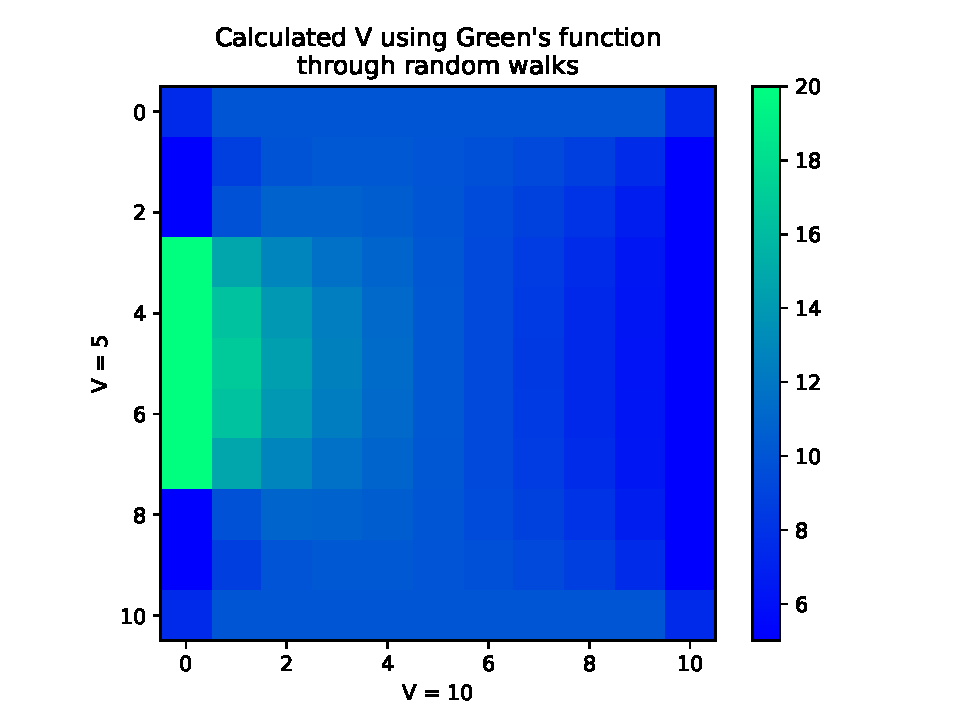
\includegraphics[scale=0.49]{img/4_4b_2_VfromG.pdf}
\end{figure}

In this configuration, $V(5, 3) = 12.61$. This makes sense since we're overriding points where $V = 5$ otherwise,
leading to points where $V = 10$ being more numerious and thus having a slightly bigger total influence compared to
the other case where we overrode points where $V = 10$, letting points where $V = 5$ have a bigger impact, relatively
speaking.

\end{document}